\documentclass{scrartcl}

\usepackage[T1]{fontenc}
\usepackage[utf8]{inputenc}

\title{Mobile Dev Week 2 Lab}
\author{Daniel Coady (102084174)}
\date{16/08/2019}

\usepackage{graphicx}

\begin{document}


\maketitle

\section*{Orientating Ourselves}
\subsection*{Task 1}
\begin{figure}[h]
    \centering
    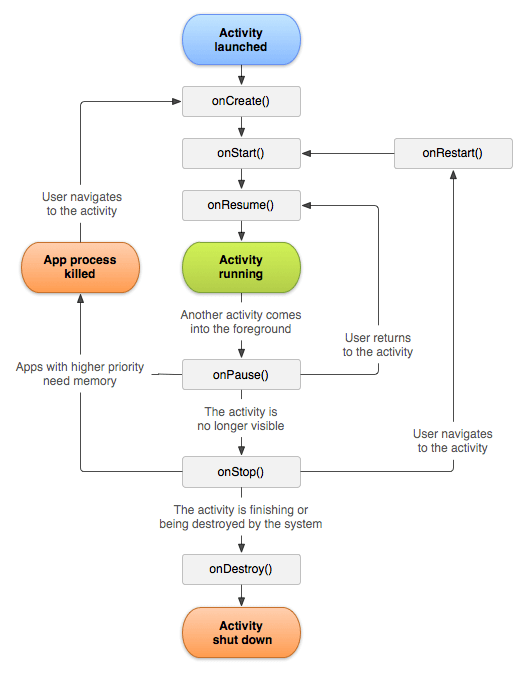
\includegraphics[scale=0.4]{images/activitylifecycle.png}
    \caption{The activity lifecycle of an app on Android}
\end{figure}
Android applications have a variety of functions that can be called when a certain event happens
on the device such as when the app is resumed or closed. This is so that the application can
handle these events appropriately without losing things like user data or progress. It's important
to consider this when developing, as seen in the application "Static Clock App" where the time
display is changed each time the orientation of the phone is changed.

\begin{figure}[h]
    \centering
    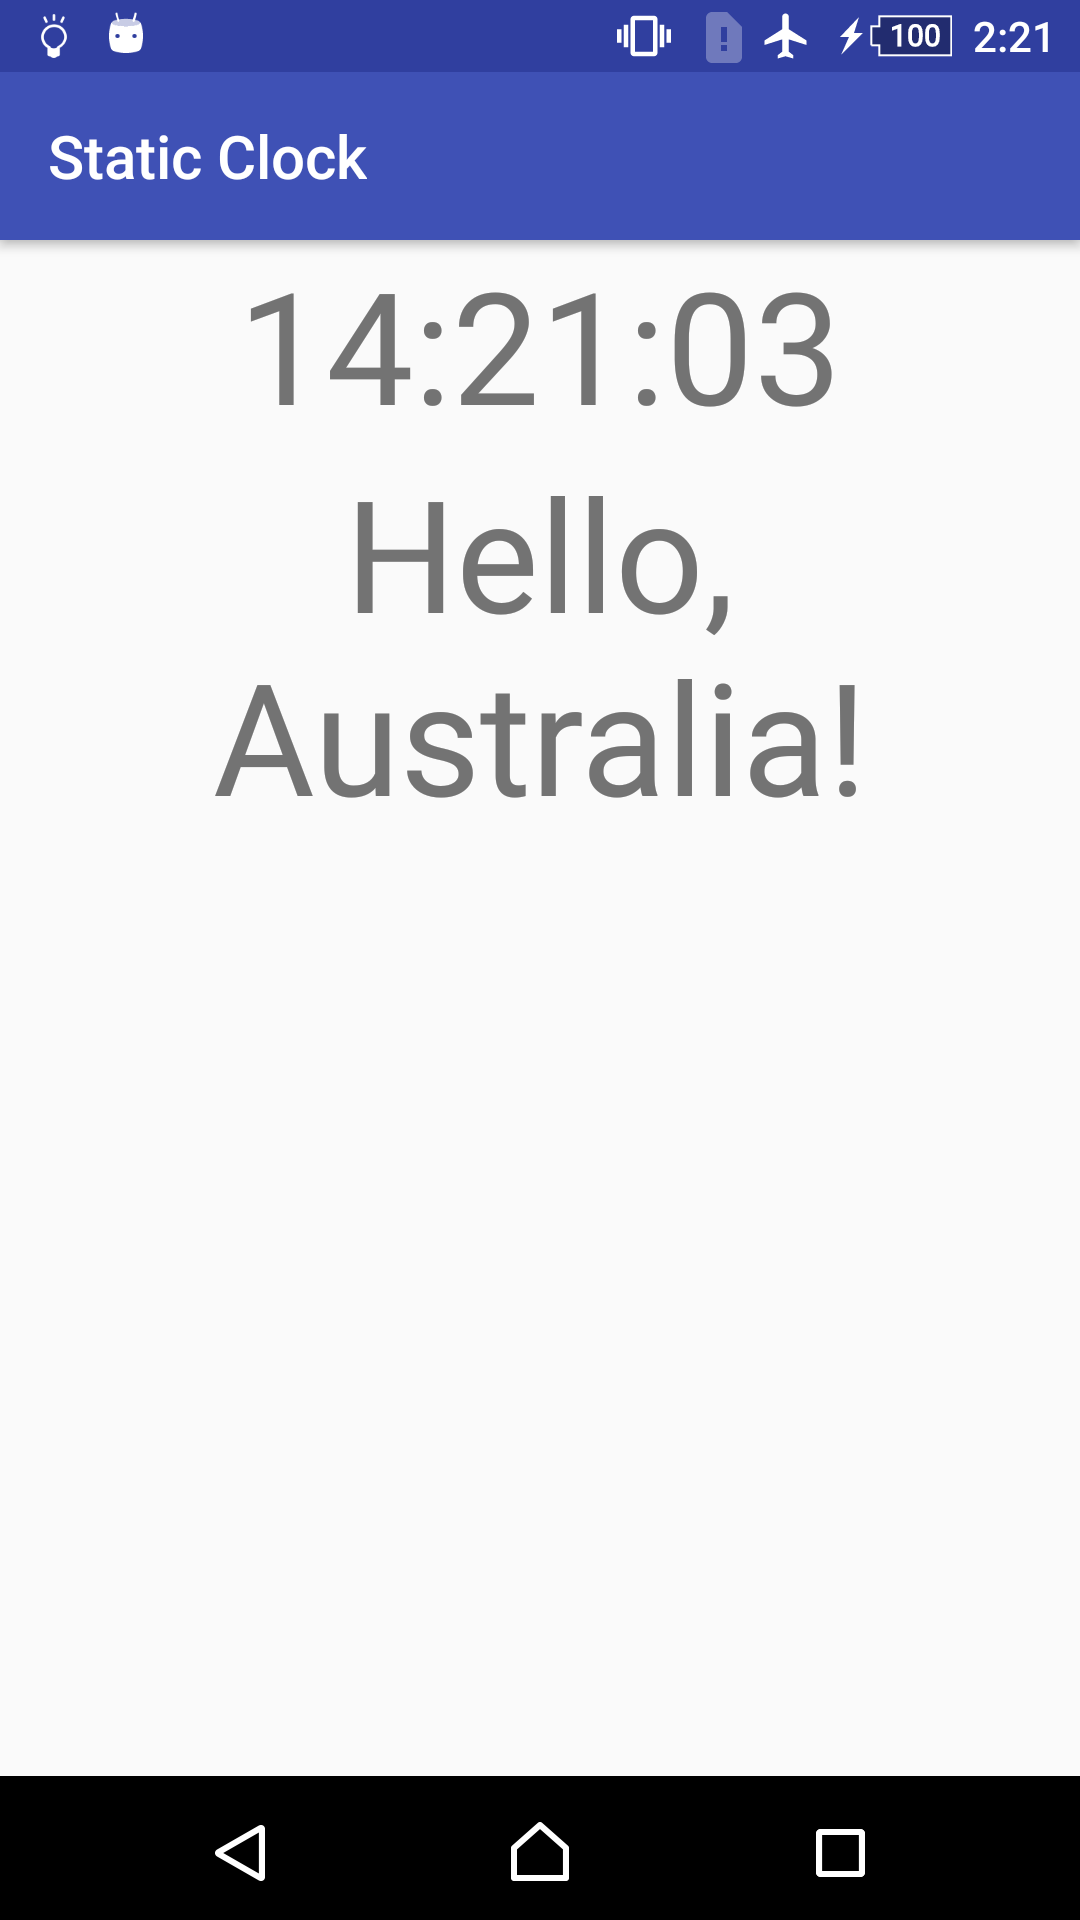
\includegraphics[scale=0.1]{images/portrait.png}
    \caption{The application in portrait}
\end{figure}
\begin{figure}[h]
    \centering
    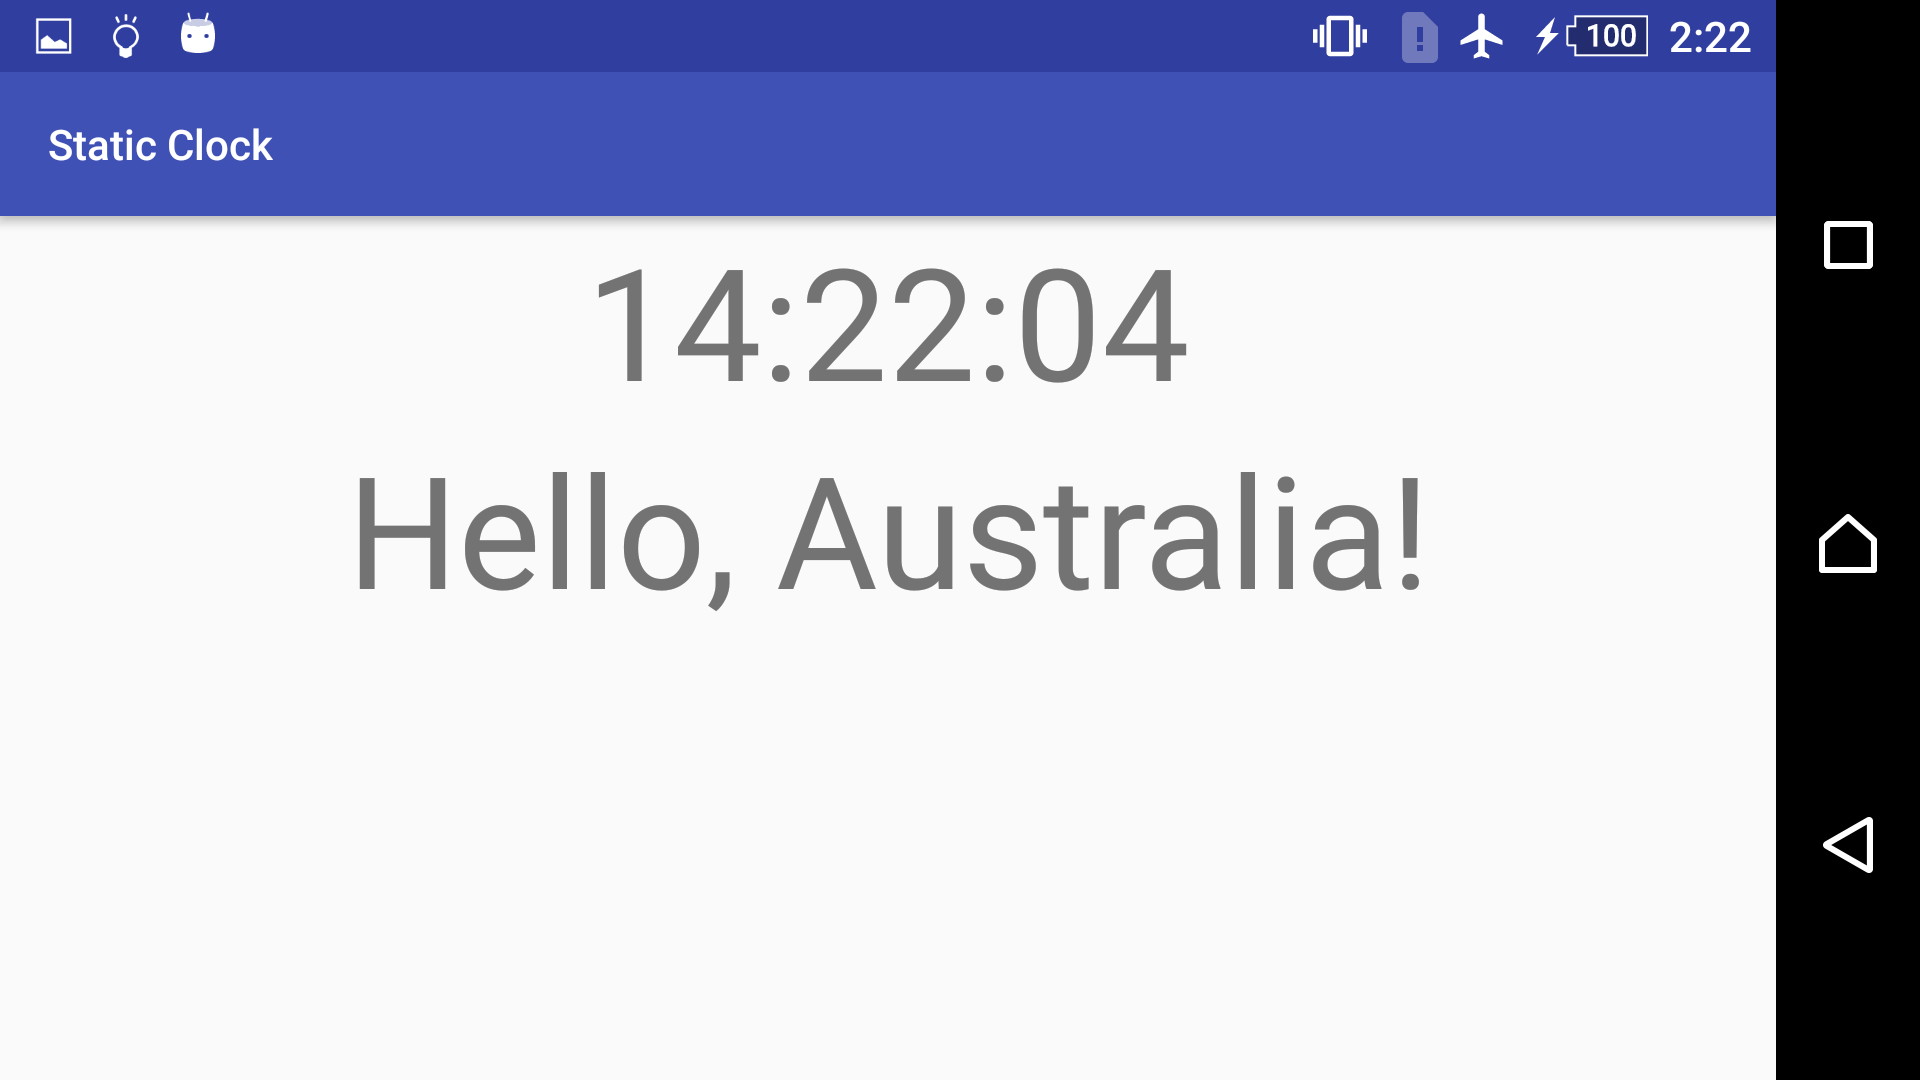
\includegraphics[scale=0.1]{images/landscape.png}
    \caption{The application in landscape}
\end{figure}

\pagebreak

This is due to what we call the "activity lifecycle" which contains some of the aforementioned
functions that are called when a certain event happens. In this case, the events are cases where
a significant state of the app changes such as when it is first launched or when it is put into
the background. In this case, we can actually see in the code itself when the time display is
handled: within the function onCreate! It's obvious then that each time the orientation changes
in the application, this function is called again which is what causes the time display to
update.

\begin{figure}[h]
    \centering
    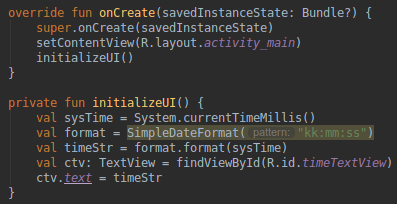
\includegraphics[scale=0.7]{images/code.png}
    \caption{The code which handles displaying the time}
\end{figure}

\begin{tabular}{p{2cm} p{11cm}}
    onResume() & When the application enters the resumed state, it brings the application to the
                 foreground and notifies all relevant sections of code that this has happened.
                 this generally occurs after the application is brought back from the background
                 (for example, a user has switched back to the application). \\[1em]
    onPause() & Paused is the state that the application will enter if put into the background
                while running. Just like the resumed state, this will notify all relevant 
                parts of the code that this has occured. \\[1em]
    onStop() & Finally, the stopped state is what the application will enter if the user fully
               exits the application. This is in many ways similar to the paused state, but with
               the key difference of an application will only enter this state if it is well and
               truly about to end and it will not continue past that. \\[1em]
\end{tabular}

\pagebreak

\subsection*{Task 2}

\begin{figure}[h]
    \centering
    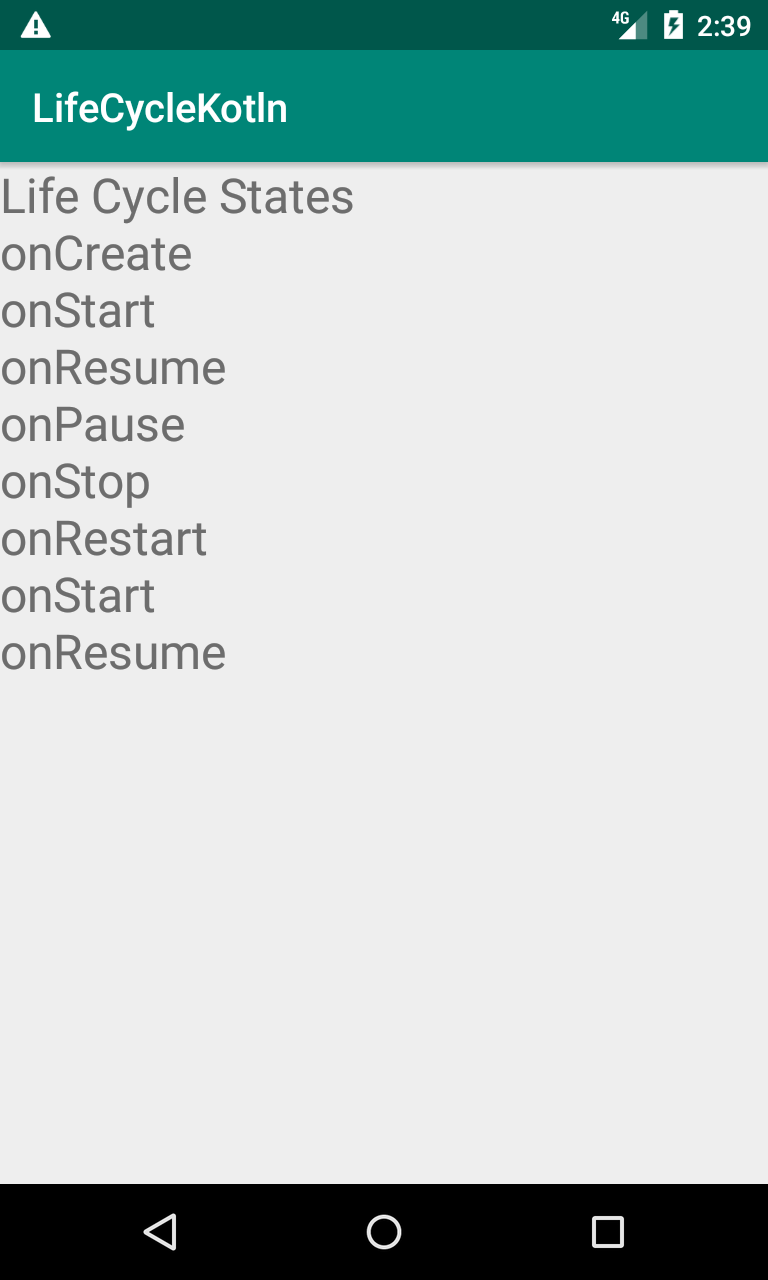
\includegraphics[scale=0.2]{images/onrestart.png}
    \caption{Triggering the on restart event}
\end{figure}

To trigger the onRestart event is quite a trivial task if you understand how the activity lifecycle
works. Looking at how it flows, you can see that to get to the activity initially running we have to
go through onCreate, onStart, and onResume. From here, the only path we then have to get to onRestart
is through onPause and then onStop. To go through these two events we can simply return to the home
screen of the phone, leaving the activity in the onStop state. There's just one more thing to do from
here, and that's to bring up the application again from the background either by opening it in the
multitasking display or by tapping on the application again. Once we do this we will go through the
onRestart event, which then leads onto the onStart and onResume events which is clearly reflected in
the screenshot of this application running.

\pagebreak

\begin{figure}[h]
    \centering
    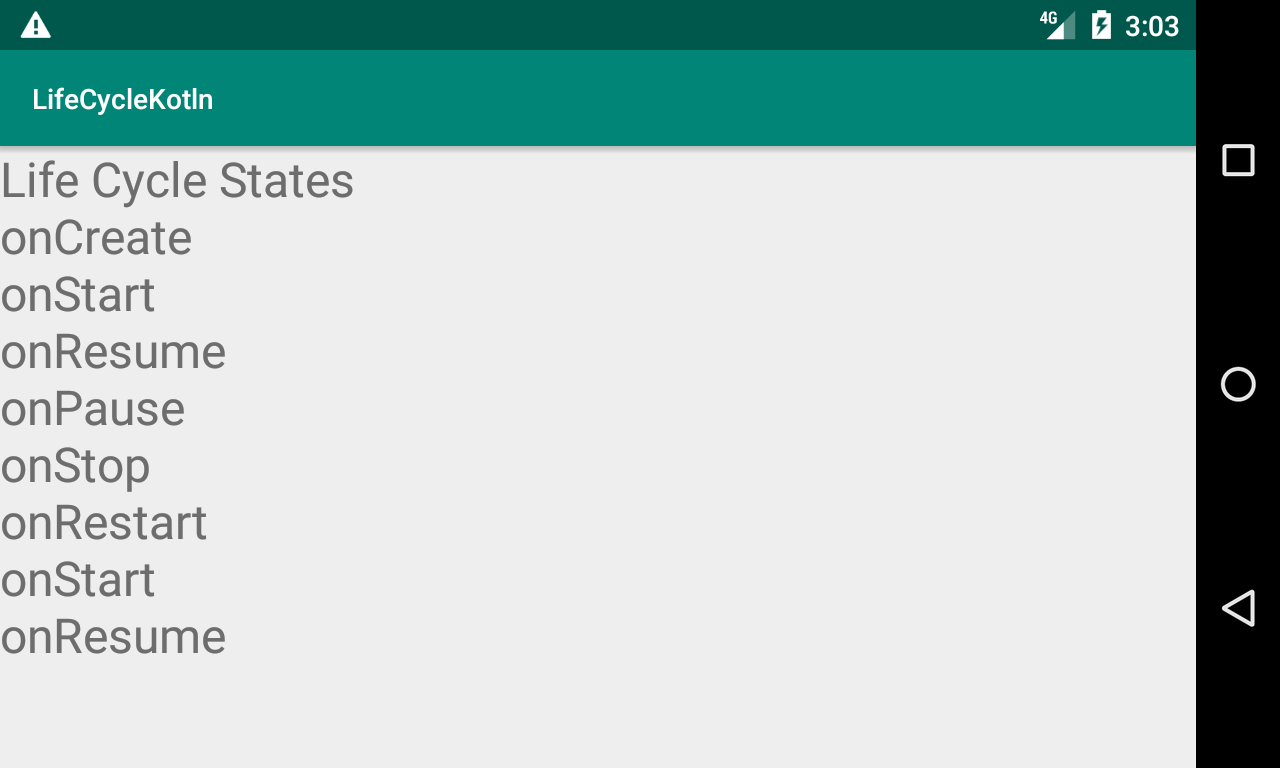
\includegraphics[scale=0.2]{images/lifecycle.png}
    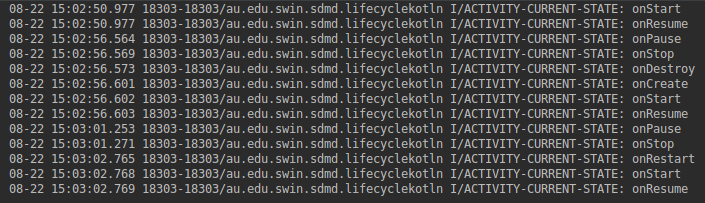
\includegraphics[scale=0.6]{images/lifecyclelog.png}
    \caption{Every event in the activity lifecycle being invoked}
\end{figure}

In this application we can see all of the events that form a part of the activity lifecycle being
invoked. However, when we look at the log and the display in the app it looks different. If you
look carefully, you can actually see that the application display doesn't show the onDestroy event
when it's called, and what's more any events invoked before are no longer displayed. This is because
when the onDestroy event is invoked the application is essentially "reset", in that it is taken back
to the onCreate event again. This means that the display is also reset and we only see the events
that have been invoked after onDestroy has happened.

\end{document}
